\newcommand{\gloss}[1]{\glossa{(#1)}}%\begin{small}\textit{(#1)}\end{small}}
\newcommand{\glossa}[1]{\begin{small}\textit{#1}\end{small}}
\newcommand{\pemph}[1]{\textbf{#1}}
\newcommand{\mmsz}{0.4\textwidth}
\newcommand{\mmultirow}[2]{\multirow{#1}{\mmsz}{#2}}

\chapter{Inducing Morphological Structure}

In this chapter, we evaluate the application of our grammar induction method to the problem of translating at the morphology level.

\section{Introduction}
Mainstream SMT research mostly ignores morphological variation, treating translation as a mapping of words and phrases from a source to a target language without taking cognisance of word-internal structure.
This approach has worked reasonably well for various languages, but is ill-suited for language pairs with substantial morphological divergence, e.g. Turkish and English.

Morphological variation is a source of sparseness in the training that can make it hard or impossible to produce correct translations of word forms not observed during training, or observed only rarely.
The sparseness problem can of course be mitigated by using ever larger sets of training data, but for anything short of an infinite parallel corpus, a language with relatively expressive morphology should succeed in producing word forms that simply never appear in the corpus.
This is especially true for languages with complex morphology like Turkish, Finnish and Hungarian, where there is a proliferation of word forms.

Ideally, we would like to leverage the words observed in the training data to generate differently inflected forms of them.
For example, the correct conjugation of the French verb for ``(we)~hear'' could be generated as illustrated below, where boldface and underlining mark the origins of the relevant word segments:

\begin{figure}[h]
%\label{fig:inflection}
\centering
	\begin{tabular}{rlcll}
	\multicolumn{2}{c}{\textbf{\textit{Observed}}} 	&  & \multicolumn{2}{c}{\textbf{\textit{Generated (not observed)}}} \\[5pt]
	\gloss{I hear} & j'\textbf{entend}s 
		&  \multirow{2}{*}{$\Longrightarrow$} 
		& \multirow{2}{*}{nous \textbf{entend}\underline{ons}} 
		& \multirow{2}{*}{\gloss{we hear}} \\ 
	\gloss{we reply} & nous r\'{e}pond\underline{ons} 	&  &  	& 
	\end{tabular} 
%\caption{Learning from morphemes: Boldface and underlining trace the elements used to form the unobserved word. English translations are given in parentheses.}
\end{figure}

In general, our aim here is to identify morphemes in the observed words and combine them correctly to generate novel word forms.
To achieve this, we require rules for how morphemes may combine.
Such rules could be hand-crafted for a particular language, but in keeping with the spirit of statistical MT, we strive toward language independent solutions and would rather induce rules from data.
A SCFG could be suitable for expressing such rules, so how about we use the grammar induction methods discussed earlier to obtain one that is capable of translating morphemes.
In particular, the plan is to have a single grammar deal with morpheme combination (i.e. word formation) as well as sentence formation.
This is the central idea for this chapter and is developed further in the next section.

\paragraph{Work this in somewhere}
Morphology has received attention in SMT research before, with reasonable success both
 when the source language has richer morphology than the target language \citep{Yang2006,Dyer2008}, 
 and vice versa \citep{someone,Yeniterzi2010} .
To our knowledge, Dyer08 is the only other case where morphology has been targeted in the context of a translation system that uses SCFG for transduction.

In the monolingual setting, morphology has been modelled with 
rule-based finite-state automata \citep{someone}, 
unsupervised methods \citep{Creutz2006,Goldsmith2001},
 .. lookup those leads from workshop feedback]. Highlight what is novel/unique about our approach.

\section{Motivation for a Labelled Grammar}
We use the Hiero-grammar with its single non-terminal category, X, as a starting point and imagine that we induce it from a corpus that has been segmented into morphemes.
For the moment, we ignore the fact that this grammar is synchronous.
Observe that a context-free grammar can be employed to generate words from morphemes, as shown by the grammar fragment and derivation of ``enabled'' in Figure \ref{fig:m_motivation_x}.

Yet the same grammar fragment also licenses the production of nonsense, such as ``enablely''.
This is because this grammar does not enforce proper restrictions on morpheme attachment, allowing a string like ``+ly address'' to attach to ``enable+'' as a `suffix'.

We use the `+' character to mark morpheme boundaries.
Apart from being a a display device, it also creates a distinction in the vocabulary if some token exists 
both as a morpheme and a word in its own right.
But it is insufficient for enforcing proper attachment, even if the grammar were aware of the marker's meaning.

\subfigcapskip=15pt
\begin{figure}[h]
  \centering
  \subfigure[Non-sensical words can be produced when using a single non-terminal category.]{\label{fig:m_motivation_x}
  \begin{tabular}{rcl}
    \begin{minipage}{0.3\textwidth}
      \begin{tabular}{lcl}
        X & $\rightarrow$ & en+ +able+ X \\
        X & $\rightarrow$ & +d \\
        \textit{X} & $\rightarrow$ & \textit{+ly address} \\
      \end{tabular}
    \end{minipage}
    &
    \begin{minipage}{0.3\textwidth}
      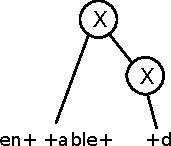
\includegraphics[scale=1]{morphology/treelet_good}
    \end{minipage}
    &
    \begin{minipage}{0.3\textwidth}
      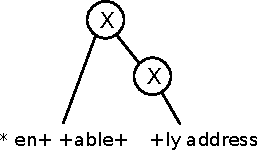
\includegraphics[scale=1]{morphology/treelet_bad} 
    \end{minipage}
    \\
  \end{tabular}
  }

  \subfigure[Constraining the grammar with labelled rules can avoid the problem.]{\label{fig:m_motivation_labelled}
  \begin{tabular}{rl}
    \begin{minipage}{0.4\textwidth}
      \begin{tabular}{lcl}
        X & $\rightarrow$ & en+ +able+ \textbf{X3} \\
        \textbf{X3} & $\rightarrow$ & +d \\
        X & $\rightarrow$ & +ly address \\
      \end{tabular}
    \end{minipage}
    &
    \begin{minipage}{0.3\textwidth}
      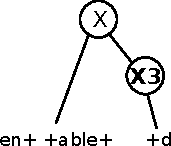
\includegraphics[scale=1]{morphology/treelet_good_label}
    \end{minipage}
    \\[10pt]
  \end{tabular}
  }
  \caption{Grammar fragments and possible derivations they allow when using a single category (top) vs. multiple categories (bottom).}
  \label{fig:m_motivation}
\end{figure}
\subfigcapskip=10pt

To solve the problem, we wish to constrain the grammar by using more refined non-terminal categories.
Specifically, we do not want the word-forming and sentence-forming rules of the grammar to mix.
Thus we propose to use a set of labelled categories for word-formation, disjoint from X.
With the modified grammar fragment shown in Figure \ref{fig:m_motivation_labelled}, the non-sensical word can no longer be produced.

These examples only serve to illustrate word formation in the monolingual case.
Of course, we are actually operating in a bilingual situation and using synchronous CFGs.
Thus, another merit of this approach is that it can capture morpheme reordering in a natural way. (Example).

\section{Morpheme Clustering and Labelling}
By no mere coincidence, we have a suitable source of the aforementioned kind of labelled grammar rules in the form of the clustering method described in chapter \ref{chap:np_clustering}.
We will use it to cluster morphemes depending on their context within words.
To this end we use the normal phrase extraction heuristics on a corpus that has been segmented into morphemes.
Thus in the terminology introduced earlier in this report, a phrase $\mathbf{p}$ and its context $\mathbf{c}$ are both sequences of morphemes, as illustrated below.
Importantly, we only perform the clustering on phrases not containing word boundaries, since we are specifically after rules of word formation.

\begin{figure}[h]
\begin{tabular}{ll}
\textit{Original sentence:}\footnote{Gloss: \gloss{changes have no place to be}} & les modifications n' ont pas lieu d' \^{e}tre \\[3pt]
\textit{Segmented sentence:} &
 $\underbrace{\textrm{les}}_{c_{-1}} \;
	\underbrace{\textrm{modifi+}}_{\mathbf{p}} \;
	\underbrace{\textrm{+cation+}}_{c_{+1}}$ \; +s n' ont pas lieu d' \^{e}tre \\[8pt]
 \multicolumn{1}{r}{$\Rightarrow$} 
 	 & $\mathbf{p}= (\textrm{modifi+}),$ \\
 	 & $\mathbf{c} = (c_{-1},c_{+1}) = (\textrm{les, +cation+})$
\end{tabular}
\end{figure}

The underlying assumption made by applying this clustering method is that a morpheme's context is indicative of its substitutability.
The previous example is an instance of noun derivation from a verb stem.
In order to form other nouns by this mechanism, different verb stems need to be substituted in place of ``modifi+''.
This can be achieved if the appropriate morphemes occurring in this context are clustered together under the same label, say, $z=15$:

\begin{center}
\begin{tabular}{ccl|ccl}
les & modifi+  & +cation+ & les & justifi+ & +cation+ \\
 & X15 &  & & X15 & \\
\end{tabular}
\end{center}

Morphemes in the training corpus are labelled in this way, based on the categories induced by clustering.
This still leaves many spans in the corpus unlabelled, in particular those that contain word boundaries.
During grammar extraction, these spans give rise to the sentence-forming X-rules, whilst the labelled spans yield the word-forming labelled rules, as detailled previously.

\section{Experimental Setup}
The ideas expressed above need to be verified empirically.
The most direct approach was to do this somewhat isolated from the other workshop experiments.
In other words, we used a Hiero-grammar as the starting point and used the clustering to learn morpheme combination rules only.
We did not also apply it to words and phrases, although that was starting to show the improved BLEU scores reported elsewhere in this document.

We chose Dutch and French as a test language pair, since 1) they both have a fair amount of interesting inflection and 2) it was the most suitable language pair from amongst those for which suitable training data was prepared before the workshop.

\subsection{System Description}

\paragraph{Data}
We filtered the training corpus down to the first 100k sentence pairs that contain at most 40 words per sentence.
The word limit was imposed because the actual number of tokens in a sentence will be higher once it is segmented into morphemes.
This was a time-saving shortcut on various fronts: It restricts the size of the extracted grammars and therefore the decoding time too, and, more importantly, allowed us to obtain the new word alignments and language model in a reasonable amount of time.
It also makes the alignment task slightly less error-prone, although this remains problematic and is discussed in section \ref{sec:m_analysis}.

\paragraph{Segmentation}
For word segmentation, we used the unsupervised Morfessor Categories-MAP algorithm \citep{Creutz2007}, which is based on a HMM.
It induces a word segmentation model from a monolingual corpus, where a word consists of one or more stem morphemes with zero or more prefixes and/or suffixes, each marked as such.
Since we weren't interested in how well Morfessor can segment words it did not observe during its training stage, we trained a segmentation model on the complete training, development and test data that will be used by the translation system.
We did not make use of the induced morpheme categories (prefix, stem, suffix), but simply applied the segmentation models to split the training, development and test data into generic morphemes.

The granularity of segmentation is controlled by specifying a perplexity threshold ($PPL$ in the Morfessor configuration file).
After some informal tests on a small data set, we chose $PPL_{\textrm{Dutch}}=300$ and $PPL_{\textrm{French}}=150$.
Table \ref{tbl:segmentation} summarises the effect this had on the (MT) training data.

\begin{table}[h]
  \centering
  \begin{tabular}{|l|l|r|r|}
    \multicolumn{2}{c}{} & \multicolumn{1}{c}{Dutch} & \multicolumn{1}{c}{French} \\ \hline
    \multirow{2}{*}{Types}  & words     & 43611 & 35225 \\ \cline{2-4}
                            & morphemes & 26409 & 21962 \\ \hline
    \multirow{2}{*}{Tokens} & words     & 2035254 & 2180898 \\ \cline{2-4} 
                            & morphemes & 2647203 & 2874574 \\ \hline
  \end{tabular}
  \caption{x}\label{tbl:segmentation}
\end{table}

\paragraph{Grammar Induction Parameters}
We obtained two grammars for testing, one by clustering the source side and the other on the target side.
Following from other workshop results, we chose $K=25$ categories, although our setting here is rather different.
Morpheme sequences of at most $|\mathbf{p}|=10$ were obtained from the aligned, segmented corpus using the standard phrase extraction method and context was chosen as one token either side of such a sequence, i.e. $\mathbf{c}=(c_{-1},c_{+1}$.
The non-parametric model with hierarchical Pitman-Yor Process priors was run for a 1000 samples in each case and the last sample used to label morpheme sequences.
The resulting grammars each have a total of 26 non-terminal categories: the default X category plus the 25 labelled categories.

\paragraph{Translation System}
Word alignments were trained on the segmented parallel corpus using the Berkeley Aligner \citep{Liang2006} with default settings.

A French language model over morpheme n-grams was also required.
3-gram language models were used throughout the workshop.
But due to word segmentation, the number of tokens in the French training corpus, and therefore the average number of tokens per sentence, increased by 32\% (Table \ref{tbl:segmentation}).
We therefore opted for a 4-gram language model, since that yields, on average, three full words of context, thus corresponding to a 3-gram model on unsegmented data.

\section{Results}

\subsection{Intrinsic Evaluation}
In order to gain some insight into the quality of the morpheme clustering, we scrutinised cluster contents for obvious patterns.
This was done only for the case where the clustering was done on Dutch (source language), since expertise was available there but not in French.
Some of the observations are summarised in Table~\ref{tbl:m_cats}. 

\begin{table}[hbt]
  \centering
    \begin{tabular}{c|p{\mmsz}|l}
    \textbf{$z$} & \textbf{Description} & \textbf{Examples} \\
                 &                      & format: $c_{-1}$ \p\ $c_{+1}$  \gloss{translation} \\ \hline
    0 & \parbox{0.4\textwidth}
        {75\% concerns the infix +s+, both as \p\ and as $c_{+1}$} &
        \begin{minipage}{0.4\textwidth}
          \begin{tabular}{ll} 
            de \pemph{europe+} +s+ & \gloss{the european+} \\
            europe+ \pemph{+s+} +e & \gloss{european}
          \end{tabular}
        \end{minipage} \\ \hline

    1 & \parbox{0.4\textwidth}
        {$>$85\% prefix morphemes as \p, mostly noun stems with plural forming $c_{+1}$.} &
        \begin{minipage}{0.4\textwidth}
          \begin{tabular}{ll} 
            ... \pemph{resolutie+} +s & \gloss{resolutions} \\
            ... \pemph{kilometer+} +s & \gloss{kilometres} \\
          \end{tabular}
        \end{minipage} \\ \hline

    4 & \parbox{0.4\textwidth}
        {$>$99\% verb stems as \p} &
        \begin{minipage}{0.4\textwidth}
          \begin{tabular}{ll} 
            ge+ \pemph{+maakt} ... & \gloss{made} \\
            ver+ \pemph{+werpt} ...& \gloss{reject(s) [verb]} \\
            samen+ \pemph{+brengt}...& \gloss{bring together} \\
          \end{tabular}
        \end{minipage} \\ \hline

    5 & \parbox{0.4\textwidth}
        {25\% \p-instances are the prefix ``ver+''. \\ 
         25\% \p-instances are the domain-specific suffix ``+missie''. \\ 
         14\% $c_{+1}$-instances are the adjective-deriving suffix ``+isch''.} &
        \begin{minipage}{0.4\textwidth}
          \begin{tabular}{ll} 
            ... \pemph{ver+} +slag & \gloss{report} \\
            ... \pemph{ver+} +beter & \gloss{improve} \\
            com+ \pemph{+missie} ... & \gloss{commission} \\
            ?? isch \\
          \end{tabular}
        \end{minipage} \\ \hline

    6 & \parbox{0.4\textwidth}
        {$>$99\% adjective stems, followed by a marker for definiteness.} &
        \begin{minipage}{0.4\textwidth}
          \begin{tabular}{ll} 
            ...\pemph{interessant+} +e & \gloss{interesting} \\
            ...\pemph{etisch+} +e & \gloss{ethical} \\
          \end{tabular}
        \end{minipage} \\ \hline

    7 & \parbox{0.4\textwidth}
        {$\pm$13\% are stems followed by ``+elijk'', often forming adverbs(?). \\
         $\pm$17\% are noun-deriving suffixes ``+heid''/``+heden''.} &
        \begin{minipage}{0.4\textwidth}
          \begin{tabular}{ll} 
            ...\pemph{aanvank+}  +elijk & \gloss{initially} \\
            ... \pemph{begrijp+}  +elijk & \gloss{understandably} \\
            vrij+  \pemph{+heden}  ... & \gloss{liberties} \\
            bevoegd+ \pemph{+heid}  ... & \gloss{authorisation} \\
          \end{tabular}
        \end{minipage} \\ \hline

    10 & \parbox{0.4\textwidth}
        {72\% full words, mostly (compound) nouns or things acting as such. Where $c_{-1}$ is an article, nouns are almost exclusively neuter singular.} &
        \begin{minipage}{0.4\textwidth}
          \begin{tabular}{ll}
            het \pemph{uit+breken}  van & \gloss{the outbreak of} \\
            ... \pemph{drie+jaren+plan}  ... & \gloss{three-year plan} \\
          \end{tabular}
        \end{minipage} \\ \hline

    16 & \parbox{0.4\textwidth}
        {$>$92\% full words, similar to but much larger than Cat. 10. Where $c_{-1}$ is an article, nouns are almost exclusively plural or male/female singular.} &
        \begin{minipage}{0.4\textwidth}
          \begin{tabular}{ll}
            de \pemph{wet+geving}  van & \gloss{the legislation of} \\
            deze  \pemph{wij+zig+ing}  ... & \gloss{this modification} \\
          \end{tabular}
        \end{minipage} \\ \hline
  \end{tabular}


  \caption{A selection of observations about the outcome of clustering morpheme sequences in the source language (Dutch). Cluster sizes ranged from X to Y.}
  \label{tbl:m_cats}
\end{table}

The quality of unsupervised clustering is generally tricky to judge.
In our case, it involves determining whether the clusters encode useful ``rules'' for morpheme combination.
There are strong indications that certain worthwhile patterns are learned and that the clustering is therefore partially successful.
To highlight some, note in Table~\ref{tbl:m_cats} that categories~4 and 6 involve a clear separation between two high-level parts of speech, and that a fine-grained distinction about Dutch nouns was learned in categories~10 and 16.

On the other hand, there are ample examples of conflation. Sometimes there is little or no useful linguistic pattern that can be discerned.
As an example, the conflation shown for category~0 implies that both ``europe+'' and ``+s'' will receive the same label, which would give rise to the kind of unrestricted substitutability that we wanted to avoid, as explained in Figure~\ref{fig:m_motivation}.

\subsection{Extrinsic Evaluation}
Ultimately, performance in translation is what matters.
The main question is what impact clustering has when applied to segmented training data.
The baseline system is therefore trained on the same segmented data but without the clustering, i.e. using the Hiero grammar.
For further comparison, we also include the score Hiero achieves on the same training data in its original, unsegmented form.

Table \ref{tbl:m_bleu} gives the final BLEU scores.

\begin{table}[htb]
  \centering
  \begin{tabular}{|l|c|c|c|} \hline
     & \textbf{OOV} & \textbf{BLEU}(m) & \textbf{BLEU} \\ \hline 
    Hiero (\textbf{baseline}) & x & 20.92  & \textbf{15.57} \\ \hline
    Source clustered & x & 20.63 & \textbf{15.37} \\ \hline
    Target clustered & x & 20.66 & \textbf{15.42} \\ \hline
    \multicolumn{3}{c}{ } \\ \hline
    Hiero, original data & x & 20.55 & \textbf{15.67} \\ \hline
  \end{tabular}
  \caption{Results, averaged over 3 MERT runs. BLEU(m) is calculated on the segmented output (i.e. the actual output in the first three cases), whereas last column contains the final scores after recombining the output morphemes into words.}
  \label{tbl:m_bleu}
\end{table}

\subsection{Analysis} \label{sec:m_analysis}
The fact that our approach degraded translation quality as measured by BLEU can be attributed to various factors.

The primary reason is that the word segmentation introduces (additional) errors into the bilingual token alignments.
The alignments are crucial, since they determine the phrases (morpheme sequences) that are extracted and input to the clustering and grammar extraction algorithms.
Alignment errors can therefore have a serious impact on the quality of the resulting grammar.

As an example of the kind of errors made, observe in Figure~\ref{fig:m_alignment_error} that morphemes from unrelated source and target words can be aligned.
Although this behaviour could be useful for modelling certain agreement phenomena or where linguistic information is expressed differently by the two languages, it causes more harm than it does good. 
In this case, it is not surprising that it mistakenly aligns the ending of the verb ``worden'' with that of the plural noun ``modifications'', since ``+en'' and ``+s'' are both plural forming suffixes and their alignment would be correct in many other contexts.
Likewise for the endings of ``niets'' (not a verb, though) and ``modifications''.
In general, it is also clear that the alignment of the segmented sentence pair is more complex than the unsegmented one, meaning there is more room for error.

\begin{figure}[hb]
  \centering
  \subfigure[Before segmentation]{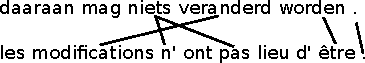
\includegraphics[scale=1]{morphology/al_orig}}
  \hspace{10mm}
  \subfigure[After segmentation]{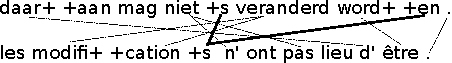
\includegraphics[scale=1]{morphology/al_segm}}
  \caption{Alignment errors increase under segmentation. (English: \glossa{Nothing may be changed about that.})}
  \label{fig:m_alignment_error}
\end{figure}

These alignment errors affect both the baseline and clustered systems.
However, the use of a single non-terminal probably allows the baseline system to recover better from bad grammar rules, due to the unrestricted substitution it licenses.
In the clustered cases, on the other hand, the grammars are more constrained by design; there is no mechanism to recover from being constrained in the wrong way, aside from the standard glue rules.

%Comparing only the Hiero-cases, we see that segmentation decreased BLEU ($15.67\to15.57$).
%Segmentation of both languages into morphemes has been shown to have this effect when using phrase-based SMT \citep{Virpioja2007}.
%However, we had expected an even larger decrease, and it might be that segmentation is less harmful in the context of hierarchical phrase-based translation (e.g. Hiero).

A further factor is that BLEU, applied in the standard way, is unforgiving towards partially correct words:
  A word with the correct stem and incorrect inflection gets penalised just the same as a wholly incorrect word.
Such partial improvements should increase the BLEU(m) score, Table~\ref{tbl:m_bleu}:
Segmentation does have this effect, but the unclustered baseline does best by this measure.

Neither the unigram scores nor the percentage of dangling morphemes in the output (i.e. ones that cannot recombine into words) improved under clustering.

On a positive note, however, clustering succeeded in correctly generating words not observed in the training, and for which the other systems failed:

\begin{table}[h]
  \begin{tabular}{llp{0.45\textwidth}}
    Input: & het ivoriaanse model & \multirow{2}{*}{\gloss{the pertaining\_to\_Ivory\_Coast model}} \\
    Reference: & du mod{\`e}le \textbf{ivoirien} \\ \hline
    Baseline:  & du mod{\`e}le \textbf{ivoir\"{i}enne} & incorrect gender \\
    Source clustered: & du \textbf{ivoirien} mod{\`e}le & correct gender, but wrong word order \\
    \phantom{.} \\
    Input: & de antidumpingmaatregelen & \multirow{2}{*}{\gloss{the anti-dumping measures}} \\
    Reference: & des \textbf{mesures antidumping}\\ \hline
    Baseline:  & \textbf{anti mesures dumping}   & correct morphemes, but bad order \\
    Target clustered: & les \textbf{mesures antidumping} & ...although +dumping+ is simply propagated as is from the Dutch input \\
  \end{tabular}
\end{table}

\section{Conclusions and Future Work}
We have presented an approach to using a Hiero-type SCFG to perform translation at the morphology level.
Context-based clustering of morpheme sequences allowed grammar rules to be constrained in way that should limit the formation of non-sensical words.

We found that clustering \textit{per se} succeeded to a large extent.
The clusters we analysed contained strong and clear patterns, learning for example a fine-grained distinction between noun gender in Dutch.

In the context of translation, our approach managed to formulate novel words that were not observed in the training data, and this was a major part of our aim.
On the whole, however, our approach degrades translation quality.

Although our translation results were negative, we would not completely discard the idea of using a SCFG in this way. 
The main problem is that segmenting the data introduces harmful errors into the word alignments.
Bad alignments mean we're screwed from the start. \textit{Thinking out loud. Tone will be fixed later...}

So we have to fix them. 

A further aspect is that translation at the morpheme level is not appropriate in all cases.
We really only want it to be used when confronting rare words or are called upon to create new ones.

A logical next step will be to combine our approach using the back-off grammar work discussed elsewhere in this report.
The idea would be to train a labelled grammar on segmented data (as we have done here) but allow back-off to a grammar trained on the unsegmented data.
This would require sentences to be input to the decoder as lattices, so that there is no hard decision about whether words or morphemes are the best granularity of representation.
This would require modifying the decoding algorithm to recombine morphemes into words when appropriate and score against a language model trained on full words.


%Future possibilities: combine with back-off grammar work, e.g. back-off from a labelled grammar (trained on segmented data) to a Hiero grammar (trained on the unsegmented data).
%express input as a lattice. That way there's no hard decision about whether to use words or morphemes. It would also require changes to decoding: e.g. morphemes will need to be combined into words whenever appropriate and scored against a LM trained on full words.
%
%need to find better solutions to the alignment problems













